\documentclass{sciposter}
\usepackage{lipsum}
\usepackage{epsfig}
\usepackage{amsmath}
\usepackage{amssymb}
\usepackage{multicol}
\usepackage{graphicx,url}
\usepackage[utf8]{inputenc}
%\usepackage{fancybullets}

\newtheorem{notation}{Notation}
\usepackage{amsthm}

\theoremstyle{definition} % amsthm only
\newtheorem{definition}{Definition}
\newtheorem{example}{Example}
\newtheorem{proposition}{Proposition}

\newcommand{\dom}{\mathrm{dom}}
\newcommand{\len}{\mathit{len}}
\newcommand{\poly}{\mathsf{poly}}

\newtheorem{algowizm}{Algorithm}
\newtheorem{theorem}{Theorem}
\graphicspath{{figures/}}


\DeclareMathOperator*{\argmin}{arg\,min}
\DeclareMathOperator*{\argmax}{arg\,max}
\newcommand{\card}[1]{\left\vert {#1} \right\vert}
	\newcommand{\apinv}[1]{\widetilde{#1}^{-1}}
\newcommand*\wc{{\mkern 2mu\cdot\mkern 2mu}}
% TODO
\usepackage[bordercolor=white,backgroundcolor=gray!30,linecolor=black,colorinlistoftodos]{todonotes}
\newcommand{\rework}[1]{\todo[color=yellow,inline]{Rework: #1}}
\newcommand{\imsize}{0.45\columnwidth}


\title{The Random Conditional Distribution}
%Título do projeto

\author{Zenna Tavares, Armando Solar Lezama}
%nome dos autores

\institute 
{MIT}
%Nome e endereço da Instituição

\email{{zenna@mit.edu, asolar@csail.mit.edu}}
% Onde você coloca os emails dos integrantes


%\date is unused by the current \maketitle

\rightlogo[1]{csaillogo}
% Exibe os logos (direita e esquerda) 
% Procure usar arquivos png ou jpg, e de preferencia mantenha na mesma pasta do .tex
%%%%%%%%%%%%%%%%%%%%%%%%%%%%%%%%%%%%%%%%%%%%%%%%%%%%%%%%%%%%%%%%%%%%%%%%%%%%%%%%
%%% Begin of Document



\begin{document}
%define conference poster is presented at (appears as footer)

\conference{{\bf ICML 2017}, Implicit Models Workshop}

%\LEFTSIDEfootlogo  
% Uncomment to put footer logo on left side, and 
% conference name on right side of footer

% Some examples of caption control (remove % to check result)

%\renewcommand{\algorithmname}{Algoritme} % for Dutch

%\renewcommand{\mastercapstartstyle}[1]{\textit{\textbf{#1}}}
%\renewcommand{\algcapstartstyle}[1]{\textsc{\textbf{#1}}}
%\renewcommand{\algcapbodystyle}{\bfseries}
%\renewcommand{\thealgorithm}{\Roman{algorithm}}

\maketitle

%%% Begin of Multicols-Enviroment
\begin{multicols}{3}

%%% Introduction
\section{Motivation}
This paper addresses approximate amortized inference in latent variable models, where (i) the prior is an implicit distribution lacking an analytical density, (ii) a known function deterministically maps latent to observable values, and (iii) most latent values are inconsistent with a given observation.
In particular, we first extend the generative adversarial framework to generate conditional samples, and then combine it with parametric inversion, a theory for inversion of non-injective functions.
This results in a method to construct a function, which we call an amortized random variable, which maps directly from an observation to a random variable whose distribution is the posterior with respect to the observation.

\section{Objectives}


\begin{enumerate}
\item To define inverse simulation when a function is not invertible.
A non-injective function $f:X \to Y$ is not invertible because it lacks a unique right inverse, a function $f^{-1}:Y \to X$ which for all $y$ satisfies:
\begin{equation}\label{eq:rightinverse}
f(f^{-1}(y)) = y
\end{equation}

\item To transform an \emph{algorithm} that implements $f$ into an inverse algorithm.

\item To apply these methods to inverse simulation of random variables for sampling from conditional probability distribution.
\end{enumerate}


\section{Parametric Inversion}

Parametric inversion generalizes function inversion to non-invertible functions.
A parametric inverse of a function $f:X \to Y$ is a parameterized function $f^{-1}:Y \times \Theta \to X$ which maps an element $y$ to a single element of its preimage: $f(y; \theta) \in \{x \mid f(x) = y\}$.
The parameter $\theta$ determines which element of the preimage is returned.

% A parametric inverse always exists.
% For example, while $f(x) = \card{x}$ is not invertible, we can define a parameter space $\theta \in \{-1,1\}$ and parametric inverse $f^{-1}(y; \theta)  = \theta \cdot y$, where $\theta$ determines whether the positive or negative inverse element is returned.


\begin{figure}
\begin{center}
         \begin{tabular}{ l | c | r }
  	$f$ & $\Theta$ & $f^{-1}$ \\
    \hline
$x+y$ & $\mathbb{R}$ & $(\theta, z - \theta)$ \\
$x-y$ & $\mathbb{R}$ & $(z + \theta, \theta)$ \\
$x\cdot y$ & $\mathbb{R} \setminus 0$ & $(z / \theta, \theta)$ \\
$x / y$ & $\mathbb{R}$ & $(z \cdot \theta, \theta)$ \\
$x^y$ & $\mathbb{R}$ & $(\theta, log_\theta(z))$ \\
$log_x(y)$ & $\mathbb{R} \setminus 0$ & $(\theta, \theta^z)$ \\
% $abs(x)$ & $\{-1,1\}$ & $\theta \cdot z$ \\
$min(x,y)$ & $\mathbb{R}^+$ & $(z, z + \theta)$ \\
$max(x,y)$ & $\mathbb{R}^+$ & $(z, z - \theta)$ \\
$sin(x)$ & $\mathbb{Z}$ & $asin(x) + 2\pi \theta$ \\
$cos(x)$ & $\mathbb{Z}$ & $acos(x) + 2\pi \theta$ \\
    \hline
\end{tabular}
\end{center}
\caption{Primitive parametric inverses.  Column $f$ contains forward non-injective functions. $\Theta$ is the parameter space used for parametric inverses shown in column $f^{-1}$. 
If a function takes multiple inputs, its parametric will return a tuple.
Parametric inverses are not unique; it is equally valid to define $\times^{-1}(z; \theta) = (z/\theta, \theta)$. }\label{tab:inverses}
\end{figure}


% An appropriate parameterisation depends on the forward function, for instance the trigonometric functions are periodic and hence naturally take an integer valued parameter, e.g. $sin^{-1}(x) = arcsin(x)+  \theta \cdot \pi$.

% As a representation of the preimage, a parametric inverse can be judged as either sound or complete.
Many functions map between a value and its preimage; we reserve the term parametric inverse for those which are sound and complete in this task.

\begin{definition}$f^{-1} : Y \times \Theta \to X$ is a sound and complete parametric inverse of $f: X \to Y$ if $\forall y$:
\begin{equation}\label{pinv}
\{ f^{-1}(y; \theta) \mid \theta \in \Theta \} = \{x \mid f(x) = y \}
\end{equation}
\end{definition}
% Condition \ref{pinv} asserts that parametric inverses are (i) sound:
% for any $\theta$, $f^{-1}(y ; \theta)$ is an element of the preimage of $y$, and (ii) complete: there exists $\theta$ corresponding to every element of the preimage.
% Inverse addition as $+^{-1}(z; \theta_1, \theta_2) = (\theta_1, \theta_2)$ is complete but not sound; for any $z$, there exists a $\theta_1$ and $\theta_2$ which sum to $z$, but there are many more pairs which do not.
% $+^{-1}(z; \theta) = (0, z)$ is sound but not complete;
% there exists no $\theta$ such that for instance $+^{-1}(0;\theta) = (-2, 2)$, despite the fact that $-2 + 2 = 0$.
% Hence, neither of these are valid parametric inverses of addition.



\section{Parametric Inversion of Composite Functions}\label{parametric-inversion-of-composite-functions}

Given functions $f_2: X \to Y$, $f_1: Y \to Z$, and composition $f=f_1 \circ f_2$, to construct  $f^{-1}:Z \times \Theta \to X$, a parametric inverse of $f$, we substitute $f_1$ and $f_2$ with their corresponding parametric inverses $f^{-1}_1$ and $f^{-1}_2$, and reverse the order of composition.

\begin{equation}\label{eq:compoverload}
f^{-1}(z;\theta_1, \theta_2) = f^{-1}_2(f^{-1}_1(z,\theta_1), \theta_2)
\end{equation}

\begin{figure}[!htb]
\centering
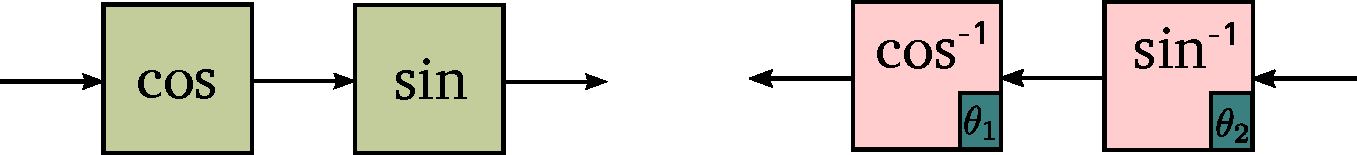
\includegraphics[width=\linewidth]{cossininvcossin.pdf}
\caption{$f = \sin \circ \cos$, then $f^{-1}(z) = \sin^{-1}(\cos^{-1}(z;\theta_1), \theta_2)$ with parameter space $\Theta = \Theta_1 \times \Theta_2$.
For most $\theta$, $\sin^{-1}(y;\theta)$ will return a value not within $[-1,1]$, the domain of $\cos^{-1}$.
$f^{-1}$ is undefined for these parameter values, and hence a \emph{partial} parametric inverse.}\label{fig:cossin}
\end{figure}

\begin{definition}If a function $f^{-1}:Y \times \Phi \to X$ does not satisfy condition $\ref{pinv}$, it is a partial parametric inverse if there exists a $\Theta \subset \Phi$ such that $f^{-1}:Y \times \Theta \to Y$ satisfies condition \ref{pinv}.
\end{definition}

\subsubsection{Composition Chains}
The procedure to invert compositions of two functions extends naturally to longer chains of composed functions.

\begin{algowizm}
\label{algo:compinversion}
Given the composition $f = f_1 \circ f_2 \cdots \circ f_n$, substitute $f_i$ with $f^{-1}_{n-i}$ to construct $f^{-1} = f^{-1}_n \circ f^{-1}_{n-1} \circ \cdots \circ f^{-1}_1$, where $f^{-1}_i$ is a parametric inverse of $f_i$.
$f^{-1}$ is a partial parametric inverse of $f$ with a parameter space $\Theta = \Theta_1 \times \Theta_2 \times \cdots \times \Theta_n$, where $\Theta_i$ is the parameter space of primitive $f^{-1}_i$.
\end{algowizm}

\subsection{Totality conditions}
Even if the forward function is total, algorithm \ref{algo:compinversion} may produce a parametric inverse which is partial.

\begin{figure}[!htb]
\centering
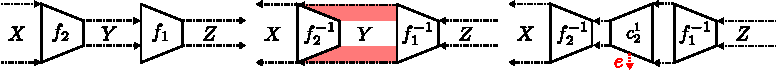
\includegraphics[width=\linewidth]{partialapprox.pdf}
\caption{The forward function (left) is a total function. Its parametric inverse (center) is partial, because there exists parameter values which generate values (in red) on which $f^{-1}_2$ is undefined. The solution used in approximate parametric inverses is to insert a restriction $c$ between the two.}\label{fig:partial}
\end{figure}

% (and not necessarily equivalent to) 
% This results in a total parametric inverse only if the output of each inverse primitive, while varying its parameter, is within the domain of the subsequent inverse primitive in the composition.

% \begin{theorem}\label{thm:invcomposition}	

\section{Approximate Parametric Inversion}\label{approximate-parametric-inversion}

An approximate parametric inverse is well defined on all values of its parameter space, but may return an incorrect inverse element unless its error value is zero.

\begin{definition}An approximate parametric inverse is a function $\widetilde{f}^{-1} : Y \times \Theta \to X \times \mathbb{R}^+$, which returns an approximate inverse element $\tilde{x} \in X$ and a non-negative error term $e \in \mathbb{R}^{+}$. $\widetilde{f}^{-1}$ is an approximate parametric inverse of $f:X \to Y$ if
$e=0$ implies $\tilde{x} \in \{x \mid f(x) = y\}$.
% , and which for all $y$ satisfies:
% \begin{equation}\label{pinv2}
% \{ f^{-1}_\Theta(y; \theta) \mid \theta \in \Theta \} \supset \{x \mid f(x) = y \}
% \end{equation}
\end{definition}



\subsubsection{Approximate Composition Chain}
\begin{algowizm}
\label{algo:approxcompinversion}
Given a partial parametric inverse $f^{-1} = f^{-1}_n \circ f^{-1}_{n-1} \circ \cdots \circ f^{-1}_1$, substitute $f^{-1}_i$ with $c_{i,j} \circ f^{-1}_i$ to construct $\apinv{f} = f^{-1}_n \circ c^{n-1}_{n} \circ f^{-1}_{n-1} \circ \cdots \circ f^{-1}_2 \circ c^1_2 \circ f^{-1}_1$.
$\apinv{f}$ is an approximate parametric inverse of $f$, where $c^i_{i-1}$ restricts values in the codomain of $f^{-1}_i$ to the domain of $f^{-1}_{i-1}$.
\end{algowizm}

\section{Conditional Sampling}

To combine parametric inversion with adversarial learning we impose constraints on the conditional generator $G$.
Rather than let $G$ be an unconstrained neural network, we use parametric inversion to construct a parameterized function family derived from $f$.

Let $f: X \to Y$ be the forward process and $f^{-1}: Y \times \Theta \to X$ be its parametric inverse.  Let $g : Y \times Z \to \Theta$ be a neural network which samples parameter values for the parametric inverse.
$G$ is then defined by composition of $f^{-1}$ and $g$:
\begin{equation}
G(y; z) = f^{-1}(y; g(y; z))
\end{equation}
To construct an amortized random variable, $G$ is trained in the adversarial sense.

\begin{figure}
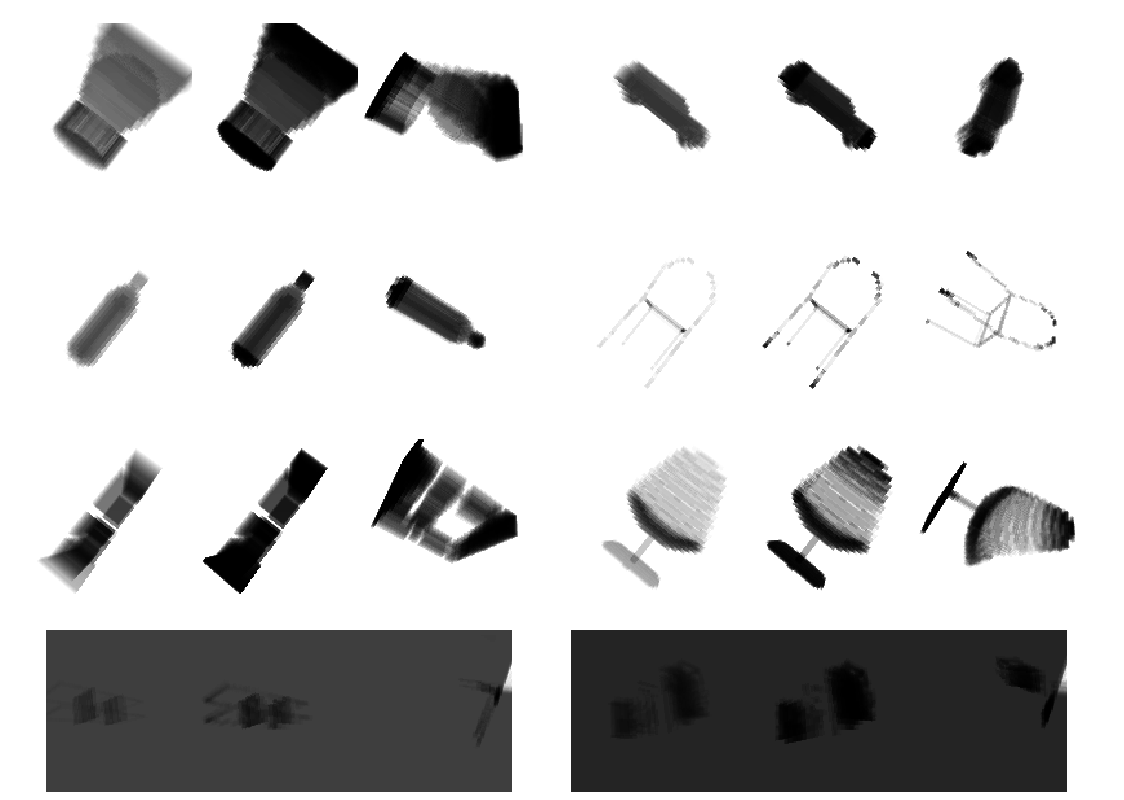
\includegraphics[width=1.0\textwidth]{inv3.png}
\caption{The left image of each triple shows our forward renderer's output given a voxel grid. The middle image results from viewing this inverted output with the same forward renderer. The right image results from viewing the inverted output at a different angle.}\label{inv_renderer}
\end{figure}



\end{multicols}

\end{document}